\documentclass[11pt,a4paper]{article}

\usepackage[T1]{fontenc}
\usepackage[utf8]{inputenc}
\usepackage[french]{babel}
\usepackage{graphicx}
\usepackage{listings}
\usepackage{xcolor}
\usepackage{array}
\usepackage[hidelinks]{hyperref}

\lstset{
    basicstyle=\ttfamily\footnotesize,
    breaklines=true,
    frame=single,
    tabsize=2,
    columns=fullflexible
}

\title{Outils de dessin vectoriel}
\author{Florian Pépin}
\date{\today}

\begin{document}

\begin{titlepage}
    \centering
    \vspace*{1.5cm}

    
\includegraphics[width=0.42\textwidth]{images/logo.jpg}

    \vspace{2.5cm}

    {\Huge\bfseries Outils de dessin vectoriel\par}

    \vspace{1.2cm}

    {\LARGE Rapport de projet\par}

    \vfill

    {\large
    Florian Pépin\\
    \vspace{0.8cm}
    \today\par}

    \vspace*{2cm}
\end{titlepage}

\tableofcontents

\newpage

\section{Patron de conception command}

\subsection{Motivation}

L'application reçoit des commandes via un CLI (Command Line Interface). Le patron Commande permet d'encapsuler chaque action dans un objet indépendant, ce qui rend l'ajout de nouvelles commandes propres et élégant.

\subsection{Correspondance des acteurs}

\begin{tabular}{|>{\raggedright\arraybackslash}p{0.34\textwidth}|p{0.54\textwidth}|}
\hline
\textbf{Acteur du pattern} & \textbf{Entité dans l'application} \\
\hline
Client & \texttt{EditMain, MergeMain et V2bmpMain} \\
\hline
Command & \texttt{EditorCommand} \\
\hline
ConcreteCommand & \texttt{RectCommand}, \texttt{CircCommand}, \texttt{SaveCommand}, etc. \\
\hline
Invoker & \texttt{Editor} \\
\hline
Receiver & \texttt{DrawingModel, V2bmpConverter, XmlSaver, XmlLoader et DrawingBuilder} \\
\hline
\end{tabular}

\begin{center}
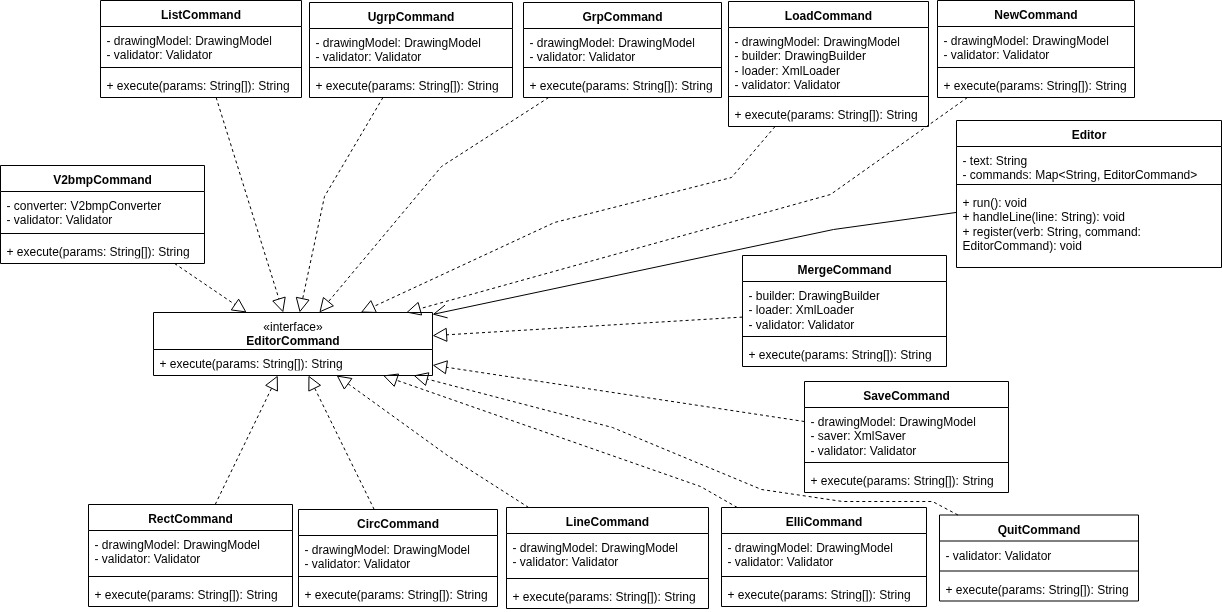
\includegraphics[width=1\textwidth]{images/UML/command.jpg}
\end{center}

\newpage

\section{Patron de conception observateur}

\subsection{Motivation}

Lorsque l'historique des formes change, la fenêtre graphique doit se mettre à jour sans que chaque commande connaisse la vue. Sans le patron Observateur, les commandes appelleraient directement \texttt{GraphicViewer}. Grâce à ce patron, \texttt{DrawingModel} notifie les observateurs après chaque changement (\texttt{fireChange}), et \texttt{GraphicViewer} réagit en repeignant le canvas : le modèle reste la source de vérité, la vue se met à jour automatiquement.

\subsection{Correspondance des acteurs}

\begin{tabular}{|>{\raggedright\arraybackslash}p{0.34\textwidth}|p{0.54\textwidth}|}
\hline
\textbf{Acteur du pattern} & \textbf{Entité dans l'application} \\
\hline
Subject & \texttt{ListenableModel} \\
\hline
ConcreteSubject & \texttt{DrawingModel} \\
\hline
Observer & \texttt{ModelListener} \\
\hline
ConcreteObserver & \texttt{GraphicViewer} \\
\hline
\end{tabular}

\begin{center}
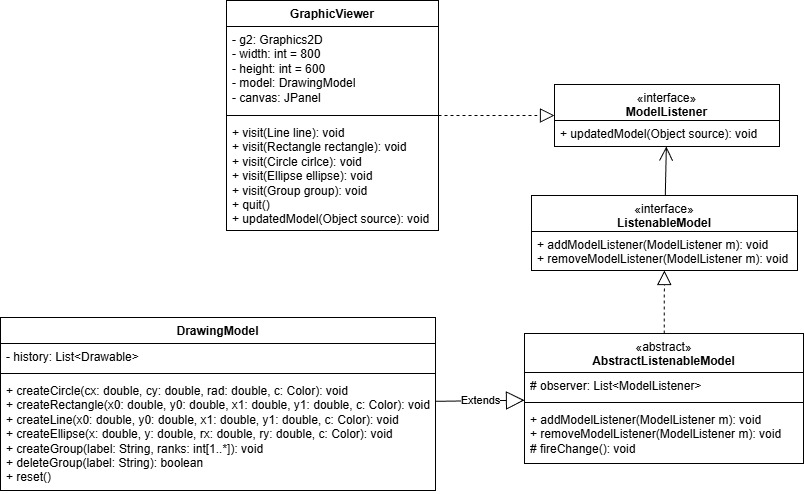
\includegraphics[width=1\textwidth]{images/UML/observer.jpg}
\end{center}

\newpage

\section{Patron de conception visiteur et composite}

\subsection{Composite : motivation}

L'application permet de regrouper des formes en groupes, eux-mêmes pouvant contenir d'autres groupes. Le Composite permet de traiter de la même manière les formes simples et les groupes.

\subsection{Composite : correspondance des acteurs}

\begin{tabular}{|>{\raggedright\arraybackslash}p{0.34\textwidth}|p{0.54\textwidth}|}
\hline
\textbf{Acteur du pattern} & \textbf{Entité dans l'application} \\
\hline
Component & \texttt{Drawable} \\
\hline
Leaf & \texttt{Rectangle}, \texttt{Circle}, \texttt{Line}, \texttt{Ellipse} \\
\hline
Composite & \texttt{Group} \\
\hline
Client & \texttt{DrawingModel}, \texttt{XmlSaver}, \texttt{GraphicViewer}, \texttt{DrawingBuilder} et \texttt{V2bmpConverter} \\
\hline
\end{tabular}

\subsection{Visiteur : motivation}

Le modèle contient différentes formes (\texttt{Rectangle}, \texttt{Circle}, \texttt{Line}, \texttt{Ellipse}, \texttt{Group}). Sans le patron Visiteur, ajouter une opération comme le rendu ou la sauvegarde XML aurait nécessité de modifier chaque classe de forme, violant le principe Ouvert/Fermé. Le Visiteur permet d'ajouter des opérations sans toucher au modèle.

\subsection{Visiteur : correspondance des acteurs}

\begin{tabular}{|>{\raggedright\arraybackslash}p{0.34\textwidth}|p{0.54\textwidth}|}
\hline
\textbf{Acteur du pattern} & \textbf{Entité dans l'application} \\
\hline
Visitor & \texttt{DrawingVisitor} \\
\hline
ConcreteVisitor & \texttt{GraphicViewer}, \texttt{XmlSaver} et \texttt{V2bmpConverter} \\
\hline
Element & \texttt{Drawable} \\
\hline
ConcreteElement & \texttt{Rectangle}, \texttt{Circle}, \texttt{Line}, \texttt{Ellipse}, \texttt{Group} \\
\hline
ObjectStructure & \texttt{DrawingModel} (liste racine) et \texttt{Group} imbriqués (listes d’enfants)\\
\hline
\end{tabular}

\begin{center}
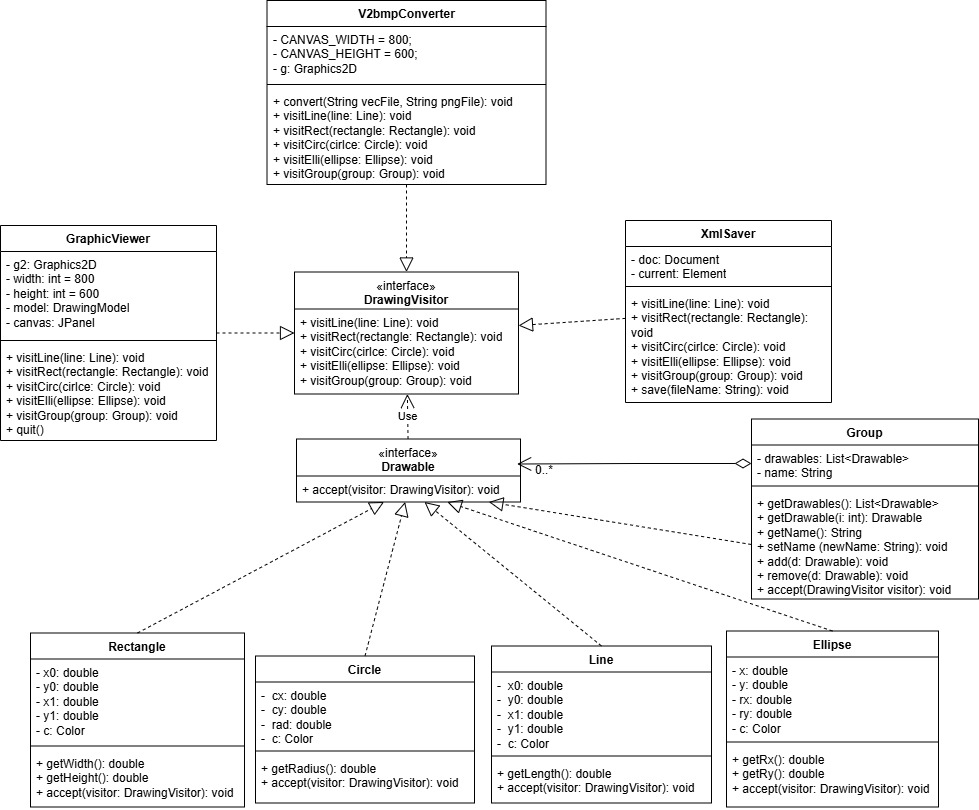
\includegraphics[width=1\textwidth]{images/UML/composite-visitor.jpg}
\end{center}

\newpage

\section{Patron de conception chaîne de responsabilité}

\subsection{Motivation}

Les commandes CLI (Command Line Interface) reçoivent des arguments sous forme de \texttt{String[]}. Il faut valider l'arité (le nombre d'arguments de la commande), le type des arguments (\texttt{double}, couleur) avant de construire la commande. Sans ce patron, chaque commande aurait géré sa propre validation. 

\subsection{Correspondance des acteurs}

\begin{tabular}{|>{\raggedright\arraybackslash}p{0.34\textwidth}|p{0.54\textwidth}|}
\hline
\textbf{Acteur du pattern} & \textbf{Entité dans l'application} \\
\hline
Handler & \texttt{Validator} \\
\hline
AbstractHandler & \texttt{ArgsValidator} \\
\hline
ConcreteHandler & \texttt{ArityValidator}, \texttt{MinArityValidator}, \texttt{DoubleValidator}, \texttt{ColorValidator} \\
\hline
Client & \texttt{Les différentes commandes} \\
\hline
\end{tabular}

\begin{center}
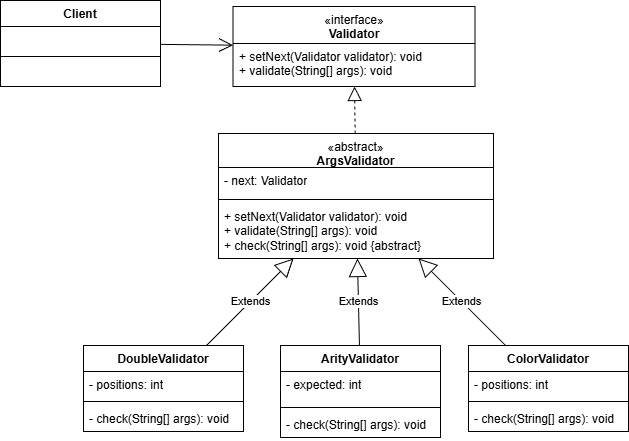
\includegraphics[width=1\textwidth]{images/UML/chains-of-responsability.jpg}
\end{center}

\newpage

\section{Patron de conception Monteur}

\subsection{Motivation}

Le chargement XML reconstruit un dessin potentiellement imbriqué (groupes dans des groupes). Le patron Monteur permet de séparer la logique de parcours du document XML (directeur) de la logique de construction du produit final (builder).\\

\texttt{XmlLoader} lit les balises et exécute les étapes de construction (\texttt{startGroup}, \texttt{setRy()}, \texttt{setCenterY()}, etc.) sans connaître la représentation finale en détail.\\

\texttt{NormalDrawingBuilder} encapsule la création concrète des \texttt{Drawable} et la gestion de la pile de groupes.

\subsection{Correspondance des acteurs}

\begin{tabular}{|>{\raggedright\arraybackslash}p{0.34\textwidth}|p{0.54\textwidth}|}
\hline
\textbf{Acteur du pattern} & \textbf{Entité dans l'application} \\
\hline
Director & \texttt{XmlLoader} \\
\hline
Builder & \texttt{DrawingBuilder} \\
\hline
Concrete Builder & \texttt{NormalDrawingBuilder} \\
\hline
Product & \texttt{List<Drawable>} \\
\hline
Client & \texttt{MergeCommand} et \texttt{LoadCommand} \\
\hline
\end{tabular}

\begin{center}
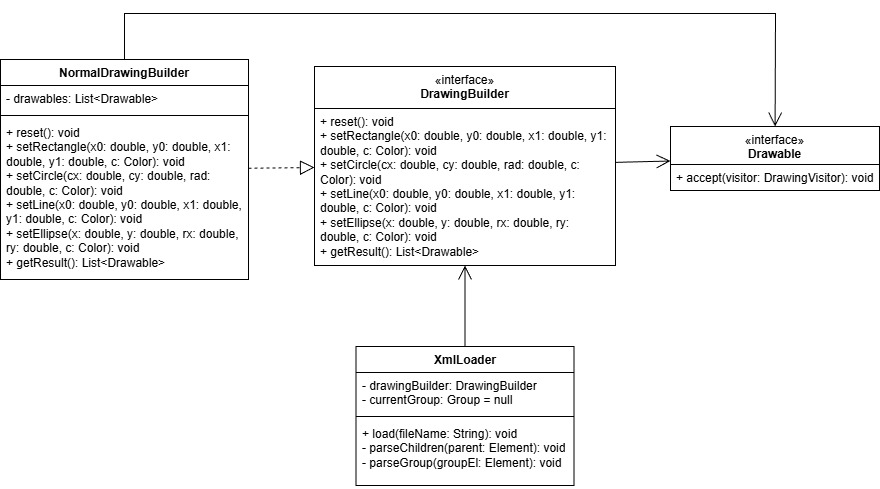
\includegraphics[width=1\textwidth]{images/UML/builder.jpg}
\end{center}

\newpage


\section{DTD XML}

\lstinputlisting{drawing.dtd}

\newpage

\section{Bilan concernant les principes d'architecture vus en cours}

L'application adopte une architecture MVC (Modèle - Vue - Controleur).\\
Cette architecture applique une séparation des responsabilités avec le modèle (\texttt{DrawingModel}, formes et groupe) qui concentre l'état et les règles métier.\\
Les différents contrôleurs (\texttt{Editor}, commandes et validation) orchestre les entrées utilisateur sans implémenter le rendu ni la persistance des données.\\
La vue (\texttt{GraphicViewer}) ne fait qu'afficher et réagit aux changements via le pattern Observeur.\\\\

Le principe SRP (Single Responsibility Principle) se voit par le fait que chaque classe a une unique responsabilité et est entièrement encapsulée.\\
Le principe OCP (Open/Close Principle) se retrouve notamment via le Visiteur et le Composite puisqu'ajouter une opération sur les formes (export, affichage) revient à écrire un nouveau visiteur sans modifier les classes de formes.\\
Le principe LSP (Liskov Substitution Principle) se retrouve via l’interface Drawable. Toute forme (Line, Rectangle, Circle, Ellipse) ainsi que le composite Group sont interchangeables. Le code client (save, parcours de l’historique, visiteurs) appelle uniquement accept(visitor) sans distinguer feuille et groupe.\\
Le principe ISP (Interface Segregation Principle) apparaît par des interfaces spécialisées : Drawable, DrawingVisitor, EditorCommand, Validator, DrawingBuilder. \\
Le principe DIP (Dependency Inversion Principle) se voit dans l’injection des abstractions. Les commandes et la vue dépendent de Drawable, DrawingVisitor, DrawingBuilder et Validator, tandis que les implémentations concrètes (XmlSaver, NormalDrawingBuilder, formes géométriques) sont fournies au niveau de l’assemblage (EditMain).\\

\newpage

\appendix

\section{Inventaire des entités par paquetage}

Liste des types publics (classes et interfaces) de l'application, regroupés par paquetage ; la colonne \emph{Rôle} résume en une phrase la responsabilité de chaque entité.

\subsection{\protect\texttt{com.drawing.controller.command}}

\begin{tabular}{|>{\raggedright\arraybackslash}p{0.36\textwidth}|p{0.56\textwidth}|}
\hline
\textbf{Entité} & \textbf{Rôle} \\
\hline
\texttt{EditorCommand} & Contrat d'une action invocable par l'éditeur avec retour d'un message pour la console. \\
\hline
\texttt{CircCommand} & Ajoute un cercle au modèle à partir des coordonnées et de la couleur fournies en arguments. \\
\hline
\texttt{ElliCommand} & Ajoute une ellipse au modèle à partir du centre, des demi-axes et de la couleur. \\
\hline
\texttt{GrpCommand} & Regroupe les formes désignées par leurs indices dans un groupe nommé. \\
\hline
\texttt{LineCommand} & Ajoute un segment au modèle entre deux points avec une couleur. \\
\hline
\texttt{ListCommand} & Retourne la représentation texte numérotée de l'historique des formes du modèle. \\
\hline
\texttt{LoadCommand} & Charge un dessin depuis un fichier XML via \texttt{XmlLoader} et le builder, puis remplace l'historique du modèle. \\
\hline
\texttt{NewCommand} & Vide l'historique du modèle pour repartir d'un dessin vierge. \\
\hline
\texttt{QuitCommand} & Demande la fermeture de la fenêtre graphique principale. \\
\hline
\texttt{RectCommand} & Ajoute un rectangle au modèle à partir de deux coins opposés et d'une couleur. \\
\hline
\texttt{SaveCommand} & Exporte tout l'historique du modèle vers un fichier XML via le visiteur XML. \\
\hline
\texttt{UgrpCommand} & Dissout le groupe situé au rang affiché par \texttt{list} lorsque cet élément est bien un groupe. \\
\hline
\texttt{MergeCommand} & Charge deux fichiers XML, les encapsule en groupes et sauvegarde le résultat fusionné dans un troisième fichier. \\
\hline
\texttt{V2bmpCommand} & Lance la conversion d'un fichier vectoriel vers une image matricielle via \texttt{V2bmpConverter}. \\
\hline
\end{tabular}

\subsection{\protect\texttt{com.drawing.controller.validation}}

\begin{tabular}{|>{\raggedright\arraybackslash}p{0.36\textwidth}|p{0.56\textwidth}|}
\hline
\textbf{Entité} & \textbf{Rôle} \\
\hline
\texttt{Validator} & Contrat d'un maillon de validation des arguments de ligne de commande. \\
\hline
\texttt{ArgsValidator} & Exécute un contrôle local puis enchaîne éventuellement le validateur suivant dans la chaîne. \\
\hline
\texttt{ArityValidator} & Vérifie que le nombre d'arguments est exactement celui attendu pour la commande. \\
\hline
\texttt{MinArityValidator} & Vérifie qu'au moins le nombre minimal requis d'arguments est présent. \\
\hline
\texttt{DoubleValidator} & Vérifie que les arguments aux indices donnés sont des nombres décimaux valides. \\
\hline
\texttt{ColorValidator} & Vérifie que les arguments aux indices donnés sont des noms de couleur reconnus par l'application. \\
\hline
\end{tabular}

\subsection{\protect\texttt{com.drawing.error}}

\begin{tabular}{|>{\raggedright\arraybackslash}p{0.36\textwidth}|p{0.56\textwidth}|}
\hline
\textbf{Entité} & \textbf{Rôle} \\
\hline
\texttt{InvalidArgException} & Exception personnalisé utile principalement pour les arguments de couleurs. \\
\hline
\end{tabular}

\subsection{\protect\texttt{com.drawing.model}}

\begin{tabular}{|>{\raggedright\arraybackslash}p{0.36\textwidth}|p{0.56\textwidth}|}
\hline
\textbf{Entité} & \textbf{Rôle} \\
\hline
\texttt{DrawingModel} & Détient l'historique des formes, applique créations et groupements, et notifie les observateurs à chaque changement. \\
\hline
\end{tabular}

\subsection{\protect\texttt{com.drawing.model.shape}}

\begin{tabular}{|>{\raggedright\arraybackslash}p{0.36\textwidth}|p{0.56\textwidth}|}
\hline
\textbf{Entité} & \textbf{Rôle} \\
\hline
\texttt{Drawable} & Contrat d'une forme géométrique du modèle acceptant un \texttt{DrawingVisitor}. \\
\hline
\texttt{DrawingVisitor} & Contrat des opérations spécifiques à chaque type de forme (patron Visitor). \\
\hline
\texttt{Line} & Modélise un segment entre deux points avec une couleur. \\
\hline
\texttt{Rectangle} & Modélise un rectangle aligné sur les axes défini par deux coins opposés et une couleur. \\
\hline
\texttt{Circle} & Modélise un cercle par centre, rayon et couleur. \\
\hline
\texttt{Ellipse} & Modélise une ellipse par centre, demi-axes et couleur. \\
\hline
\texttt{Group} & Modélise un composite regroupant plusieurs \texttt{Drawable} sous un nom. \\
\hline
\end{tabular}

\subsection{\protect\texttt{com.drawing.model.builder}}

\begin{tabular}{|>{\raggedright\arraybackslash}p{0.36\textwidth}|p{0.56\textwidth}|}
\hline
\textbf{Entité} & \textbf{Rôle} \\
\hline
\texttt{DrawingBuilder} & Contrat du builder : construction par étapes (\texttt{begin*} $\rightarrow$ setters $\rightarrow$ \texttt{build()}) et gestion des groupes imbriqués. \\
\hline
\texttt{NormalDrawingBuilder} & Implémentation concrète du builder avec état \texttt{ShapeKind} et pile de groupes. \\
\hline
\texttt{ShapeKind} & Énumération du type de forme en cours de construction (\texttt{NONE}, rectangle, cercle, ligne, ellipse). \\
\hline
\end{tabular}

\subsection{\protect\texttt{com.drawing.model.xml}}

\begin{tabular}{|>{\raggedright\arraybackslash}p{0.36\textwidth}|p{0.56\textwidth}|}
\hline
\textbf{Entité} & \textbf{Rôle} \\
\hline
\texttt{XmlLoader} & parse le XML et pilote le \texttt{DrawingBuilder} pour construire les formes. \\
\hline
\texttt{XmlSaver} & parcourt les \texttt{Drawable} et construit un arbre DOM XML. \\
\hline
\end{tabular}

\subsection{\protect\texttt{com.drawing.model.converter}}

\begin{tabular}{|>{\raggedright\arraybackslash}p{0.36\textwidth}|p{0.56\textwidth}|}
\hline
\textbf{Entité} & \textbf{Rôle} \\
\hline
\texttt{V2bmpConverter} & charge un fichier \texttt{.vec} via \texttt{XmlLoader} et rasterise le dessin en image PNG. \\
\hline
\end{tabular}

\subsection{\protect\texttt{com.drawing.util}}

\begin{tabular}{|>{\raggedright\arraybackslash}p{0.36\textwidth}|p{0.56\textwidth}|}
\hline
\textbf{Entité} & \textbf{Rôle} \\
\hline
\texttt{ListenableModel} & Contrat d'un modèle pouvant enregistrer et retirer des observateurs sur ses changements. \\
\hline
\texttt{ModelListener} & Contrat d'un observateur appelé après une mutation du modèle. \\
\hline
\texttt{AbstractList\-enable\-Model} & Fournit la liste d'observateurs et la notification \texttt{fireChange} aux modèles dérivés. \\
\hline
\texttt{ColorDecode} & Traduit les noms de couleur texte en \texttt{Color} et inversement pour la console et l'XML. \\
\hline
\end{tabular}

\subsection{\protect\texttt{com.drawing.view}}

\begin{tabular}{|>{\raggedright\arraybackslash}p{0.36\textwidth}|p{0.56\textwidth}|}
\hline
\textbf{Entité} & \textbf{Rôle} \\
\hline
\texttt{GraphicViewer} & Fenêtre Swing qui dessine l'historique du modèle et se met à jour lorsque le modèle notifie un changement. \\
\hline
\end{tabular}

\subsection{\protect\texttt{com.drawing}}

\begin{tabular}{|>{\raggedright\arraybackslash}p{0.36\textwidth}|p{0.56\textwidth}|}
\hline
\textbf{Entité} & \textbf{Rôle} \\
\hline
\texttt{EditMain} & Point d'entrée dédié à l'éditeur de dessin. \\
\hline
\texttt{MergeMain} & Point d'entrée dédié à la commande \texttt{merge} (fusion de deux dessins XML). \\
\hline
\texttt{V2bmpMain} & Point d'entrée dédié à la commande \texttt{v2bmp} (conversion vectoriel vers PNG). \\
\hline
\end{tabular}

\subsection{\protect\texttt{com.drawing.controller}}

\begin{tabular}{|>{\raggedright\arraybackslash}p{0.36\textwidth}|p{0.56\textwidth}|}
\hline
\textbf{Entité} & \textbf{Rôle} \\
\hline
\texttt{Editor} & Lit les lignes saisies, dispatche le verbe vers le registre et affiche le message renvoyé par la commande exécutée. \\
\hline
\end{tabular}

\end{document}
